\section{Auswertung}
\label{sec:Auswertung}


\begin{table}
  \caption{Kanäle mit vom Doppelimpulsgenerator vorgegebenen Zeitintervallen sowie ihr Abstände}
  \label{tab:Kalibrierung}
  \centering
  \sisetup{round-mode = places , round-precision = 2,scientific-notation=fixed, fixed-exponent = 0}
  \begin{tabular}{|S|S|}
    \toprule
    Kanal & Abstand \\
    \midrule
    0.            &  \\
    22.16501487   & 22.16501487 \\
    44.95410911   & 22.78909424 \\
    67.           & 22.04589089 \\
    89.           & 22 \\
    111.          & 22 \\
    133.          & 22 \\
    155.          & 22 \\
    177.          & 22 \\
    199.          & 22
    \bottomrule
  \end{tabular}
\end{table}

Aus den in Tab. \ref{tab:Kalibrierung} aufgeführten Werten (gemittelt aus Tab. \ref{tab:kanal} nach \eqref{eq:kanal}) ergibt sich eine Umrechnung von $22.11 \pm 0.08 \, \frac{\text{Kanäle}{\si{\micro\second}}}$.


Fit:
403+/-9 Amplitude
2.02+/-0.04 tau/microseconds
2.85+/-0.29 untergrund

fit mit sigma = sqrt(C)

% \begin{figure}
%   \centering
%   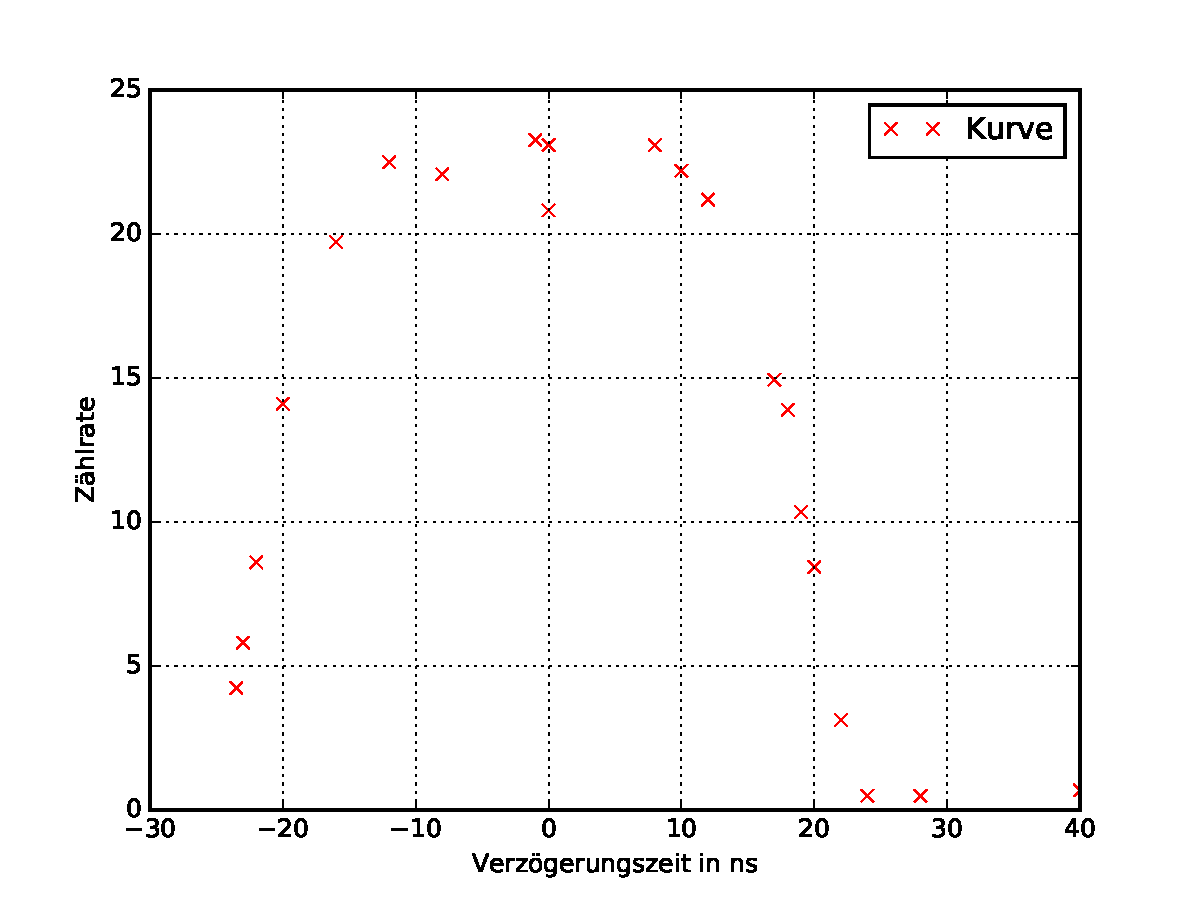
\includegraphics{plot.pdf}
%   \caption{Plot.}
%   \label{fig:plot}
% \end{figure}



% \begin{table}
%    % Notation :  {% nicht entfernen ist sehr wichtig sonst Fehler !!
% \parbox{0.48\textwidth}{% %Ermöglicht zwei Tabellen neben einander
%   \centering
%   \sisetup{round-mode = places , round-precision = 0,scientific-notation=fixed, fixed-exponent = 0}
%          %rundet Werte aus Stelle, Stelle = ,  macht einen bestimmten festen exponenten
%   \resizebox{\textwidth}{!}{%  % skaliert zu große Tabellen
%   \begin{tabular}{S@{${}\pm{}$} S} % fügt plus minus Fehler Schreibweise hinzu
%     \toprule
%      $\text{e}_b / \si{\milli\meter}$ &
%      $\text{d}_b /\si{\milli\meter} $ & $\text{f}_b / \si{\milli\meter} $\\
%     \midrule
%     \bottomrule
%   \end{tabular}
%   % }
%   \caption{Tabellenunterschrift}
%   \label{tab:tab}
% }
% % \end{table}
% % \begin{table}
% \parbox{0.48\textwidth}{%
%   \centering
%   \sisetup{round-mode = places , round-precision = 0,scientific-notation=fixed, fixed-exponent = 0}
%   % \resizebox{\textwidth}{!}{%
%   \begin{tabular}{S@{${}\pm{}$} S}
%     \toprule
%      $\text{e}_b / \si{\milli\meter}$ &
%      $\text{d}_b /\si{\milli\meter} $ & $\text{f}_b / \si{\milli\meter} $\\
%     \midrule
%     \bottomrule
%   \end{tabular}
%   % }
%   \caption{Tabellenunterschrift}
%   \label{tab:tab}
% }
% \end{table}
